
% This template has been edited from the IEEE template available at:
% https://www.ieee.org/conferences/publishing/templates.html
%
% For further help, you may wish to see:#
% https://www.overleaf.com/learn/latex/tables
% https://www.overleaf.com/learn/latex/Inserting_Images
% https://www.overleaf.com/blog/532-creating-and-managing-bibliographies-with-bibtex-on-overleaf

\documentclass[conference]{IEEEtran}
%\IEEEoverridecommandlockouts
% The preceding line is only needed to identify funding in the first footnote. If that is unneeded, please comment it out.
\usepackage[a4paper, total={6in, 8in}, margin=0.75in]{geometry}
\usepackage{cite}
\usepackage{amsmath,amssymb,amsfonts}
\usepackage{algorithm} 
\usepackage{algpseudocode} 
\usepackage{graphicx}
\usepackage{textcomp}
\usepackage{xcolor}
\usepackage{color,soul}
\usepackage{float} % to allow figures across 2 columns

\def\BibTeX{{\rm B\kern-.05em{\sc i\kern-.025em b}\kern-.08em
    T\kern-.1667em\lower.7ex\hbox{E}\kern-.125em}}
\begin{document}

\title{Achieving Accurate Odometry Through Self-Calibration - A Robot's Quest to Find Itself}

\author{
    \IEEEauthorblockN{1902072}
    \and
    \IEEEauthorblockN{1839288}
}

\maketitle

\begin{abstract}

This report investigates the challenges of achieving accurate odometry in autonomous mobile robots, specifically the Pololu 3Pi+ robot. 
By examining the effectiveness of an automated calibration circuit to measure key robot dimensions, this study aims to determine whether such calibration can significantly reduce systematic odometry errors compared to using default dimensions. 
The findings reveal that the proposed calibration method can detect variations in wheel radii and wheelbase dimensions, and the adjustments made through automated calibration improve the robot's odometry accuracy and precision. 
The proposed calibration procedure has potential applications for efficiently calibrating large numbers of robots for industrial use or swarm robotics.
\end{abstract}


\section{Introduction}\label{sec:intro}

The use of mobile robotics in industry is becoming more common for logistics, deliveries and manufacturing.
One of the key challenges when deploying autonomous mobile robots is accurate odometry, which is the process of using sensor data and robot kinematics to calculate the position of the robot over time.

Accurate odometry aims to reduce systematic errors, caused by inaccuracies in robot dimensions, sensors or actuators. Non-systematic errors are random errors caused by variations in the robot's environment and are generally less critical as they do not accumulate over time.
Typically, the literature reflects wheel radius and wheelbase measurement errors as the most common sources of systematic odometry error \cite{UMBmark, width-radius}, and precise measurement of these dimensions can be difficult to achieve.

Slight variations in dimensions between robots, due to manufacturing and assembly tolerances, may require individual calibration for each robot to be accurate.
This is often achieved through manual trial-and-error-based calibration, a slow process prone to user error which is impractical for large swarms of robots. 
Without this, well-programmed robots will produce precise but potentially inaccurate results when tested for linear and orientation accuracy.

This report develops an automatic calibration circuit and method to measure the key dimensions of a Polulu 3Pi+ robot using its onboard sensors and processors, aiming to reduce the need for time-consuming manual adjustments. 

\begin{figure}[h!]
    \centering
    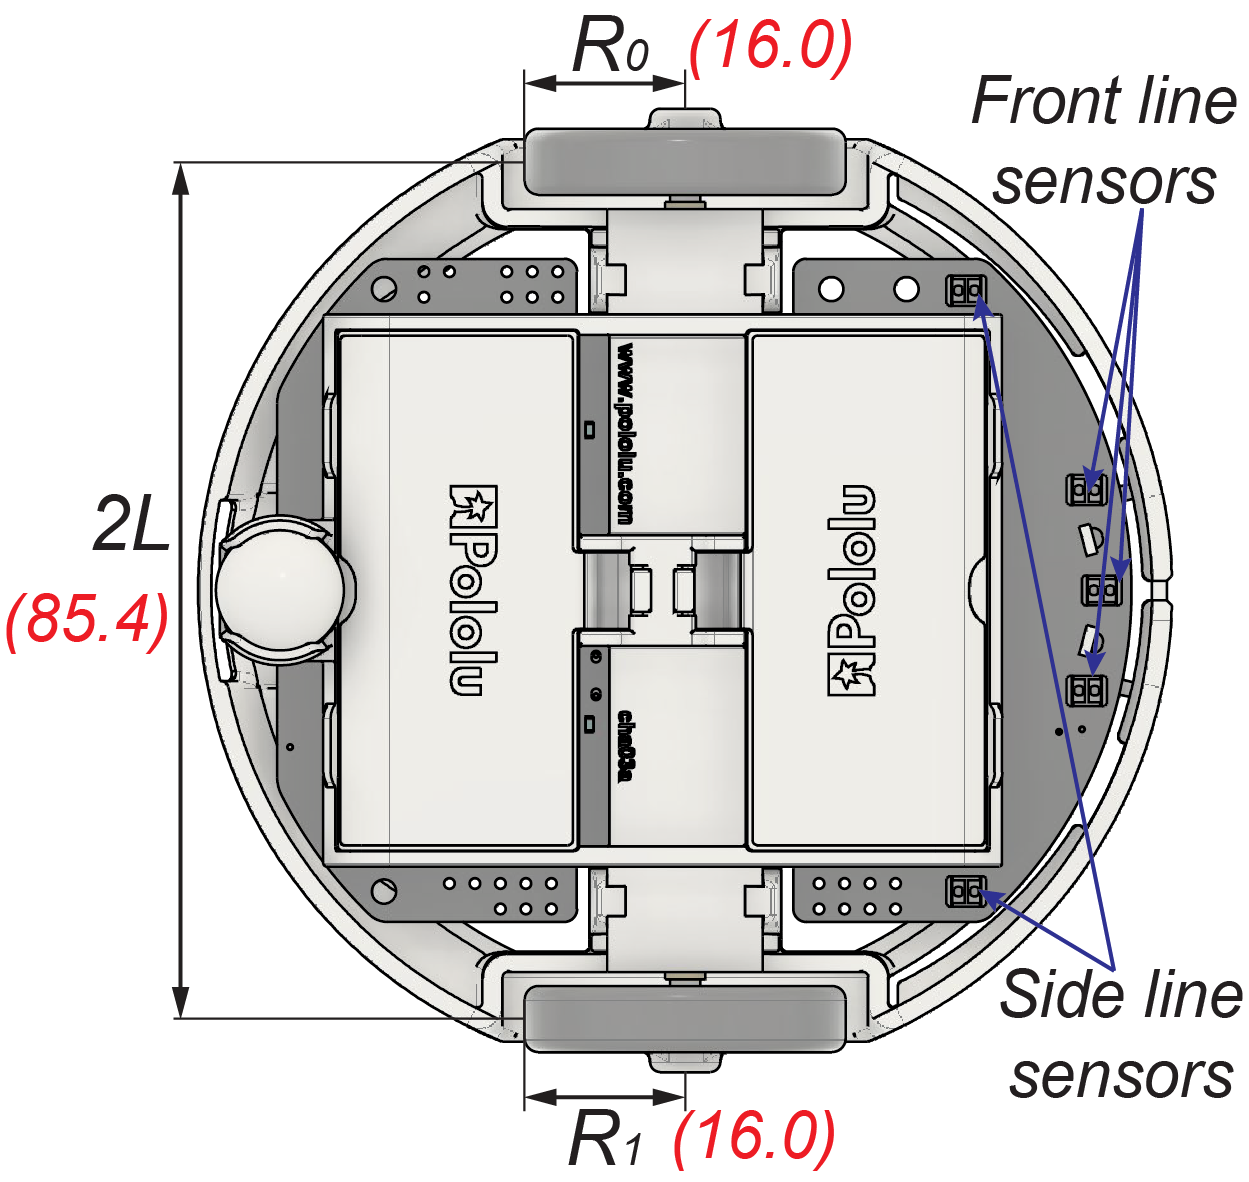
\includegraphics[width = 0.49\textwidth]{img/robot_schemtatic.png}
    \caption{Bottom view of the Pololu 3Pi+ CAD model with dimensions \cite{pololu_guide}}
    \label{fig:dimensions}
\end{figure}

Among the 3Pi+'s extensive range of sensors, the robot contains wheel encoders and infrared-radiation (IR) sensors \cite{pololu_guide}. 
The two key dimensions used in the differential drive kinematics model are the width of the wheelbase and the wheel radii \cite{pololu_guide}, shown in Figure \ref{fig:dimensions}.


\subsection{Hypothesis Statement}

As part of this study, there are two key hypotheses related to robot calibration. The first is that individual robots require individual calibration to achieve the same odometry accuracy. The second hypothesis is that individual calibration can be achieved through an automatic one-time offline calibration using a calibration circuit.

\begin{quote}
    \emph{
    The authors hypothesize that variances in wheel diameter and wheelbase width significantly affect the odometry accuracy of the Pololu 3Pi+ robot.
    This experiment predicts that a calibration circuit and method using onboard sensors can automatically measure the wheel radii and wheelbase.
    By applying this calibration, we anticipate a measurable improvement in odometry accuracy through a reduction in systematic errors when compared to performance using the default dimensions from the datasheet.
    }
\end{quote}


% These hypothesese will be tested by two accuracy tests on the robot. 
% The hypothesis will be enacted by creating a calibration code that works on a predefined test circuit, and then the robot is tested using both the UMBmark test and a straight line distance. 
% The first test will confirm the heading angle (theta) error and the second will confirm a distance error. 
% If both of these tests indicate a better performance after calibration then the hypothesis will be accepted.

% By minimising the human interaction required this process can be made quicker and cheaper, hence the use of automated measurements on a pre-designed circuit.


\section{Implementation}\label{sec:implementation}

The system's odometry accuracy is evaluated against two tests: linear distance and orientation angle. 
Initially, these tests were conducted on the uncalibrated system, using the default dimensions provided in the 3Pi+’s datasheet for the kinematic model. This establishes a baseline for performance.

Next, the robot was run on a printed calibration test circuit, using line sensor feedback to determine robot-specific dimensions. 
These dimensions are updated in the kinematic model \cite{paul} and the calibrated system is re-tested to determine if there is an improvement in odometry accuracy.

\paragraph{Linear accuracy} The linear accuracy is tested by measuring a known distance using the 3Pi+'s line sensors and comparing the measured value to the true distance.
The robot is driven in a straight line at a constant 70mm/s across two marked points spaced 500mm apart.
The robot records the number of wheel rotations (N) between the tick marks, measured by the encoders, and calculates the distance travelled using:

\begin{equation}
    D = 2 \pi R N
\end{equation}

The distance measurement is taken between the two rising edges of the line sensor's detection signal, shown in Figure \ref{fig:linesensor}.
This aims to minimise any variation in distance measurements caused by changes in ambient light, which affects how early the sensor line detection threshold is crossed.
If the reading was taken from the two outside edges of the tick marks (rising edge to falling edge) then differences in ambient lighting would affect the distance measured.

\begin{figure}[h!]
    \centering
    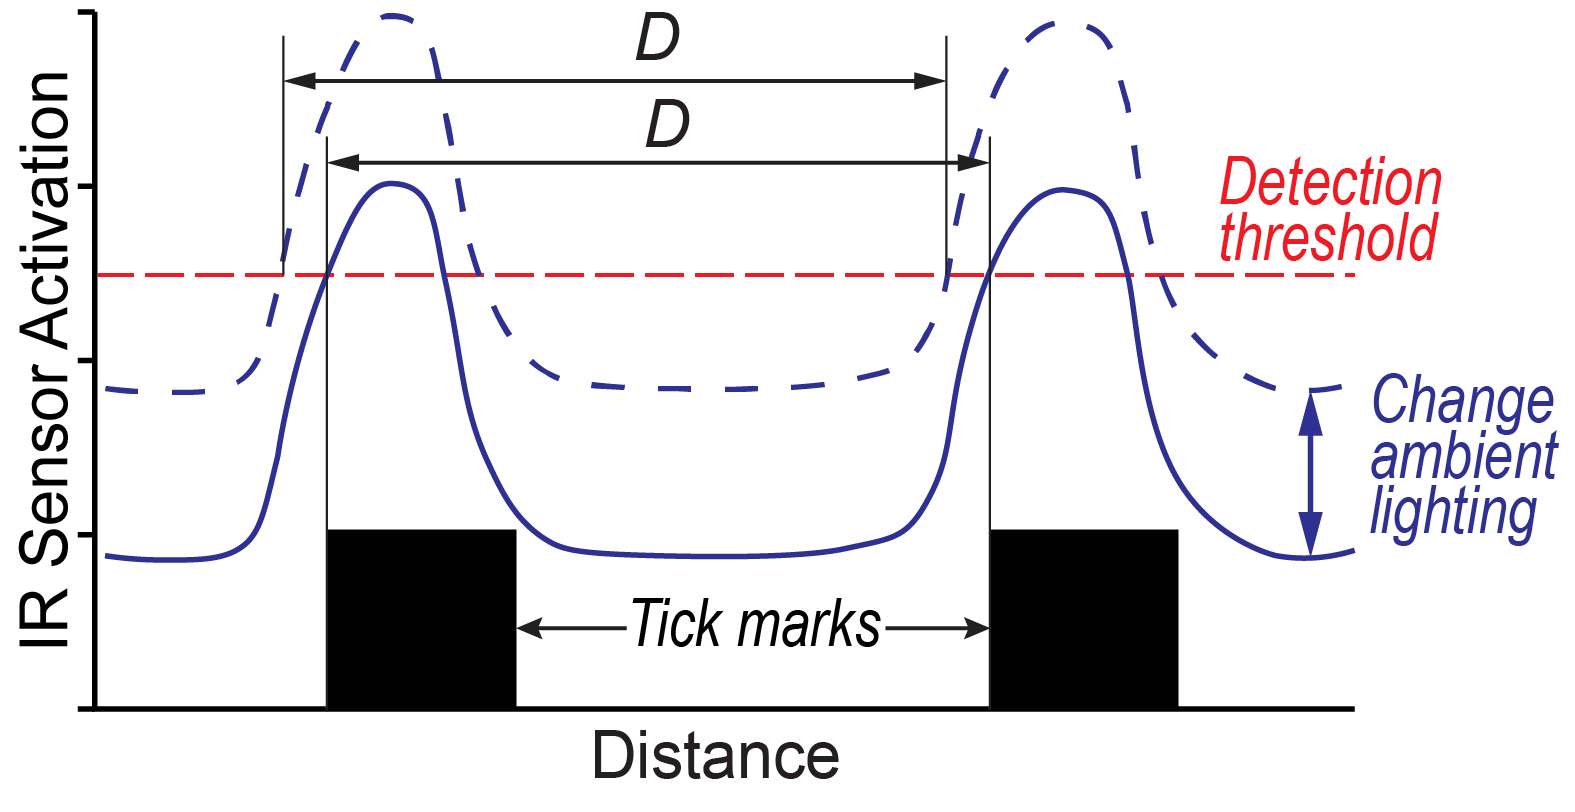
\includegraphics[width = 0.49\textwidth]{img/linesensor_response.png}
    \caption{Line sensor response and activation threshold}
    \label{fig:linesensor}
\end{figure}

\paragraph{Orientation accuracy}
The orientation accuracy of the robot is measured using the UMBmark test \cite{UMBmark}. 
The robots complete two circuits around a 0.5m x 0.5m square and the orientation and distance error from the origin are recorded on completion.
The line sensors are not used during this test. The robot drives at 70mm/s and turns on the spot for each 90-degree corner, then stops once it has reached its internal origin.
At the end of the test, the location and orientation of the robot are marked, and the x and y errors from the true origin are measured using a ruler.
The orientation error from the x-axis was measured using a digital angle gauge.
By completing two laps, the systematic error is amplified, making it easier to measure precisely. 
The test is run both clockwise (CW) and counter-clockwise (CCW) to distinguish between systematic errors that cancel each other out.

\paragraph{Calibration}
A test circuit was designed to calibrate the 3Pi+’s kinematics, shown in Figure \ref{fig:calibration_circuit}. 
The line sensors are used to control the movement of the robot along the pre-defined printed path, allowing the deviation between the kinematic model and the true circuit dimensions to be used to calculate the wheel radii and the wheelbase length.

\begin{figure}[h!]
    \centering
    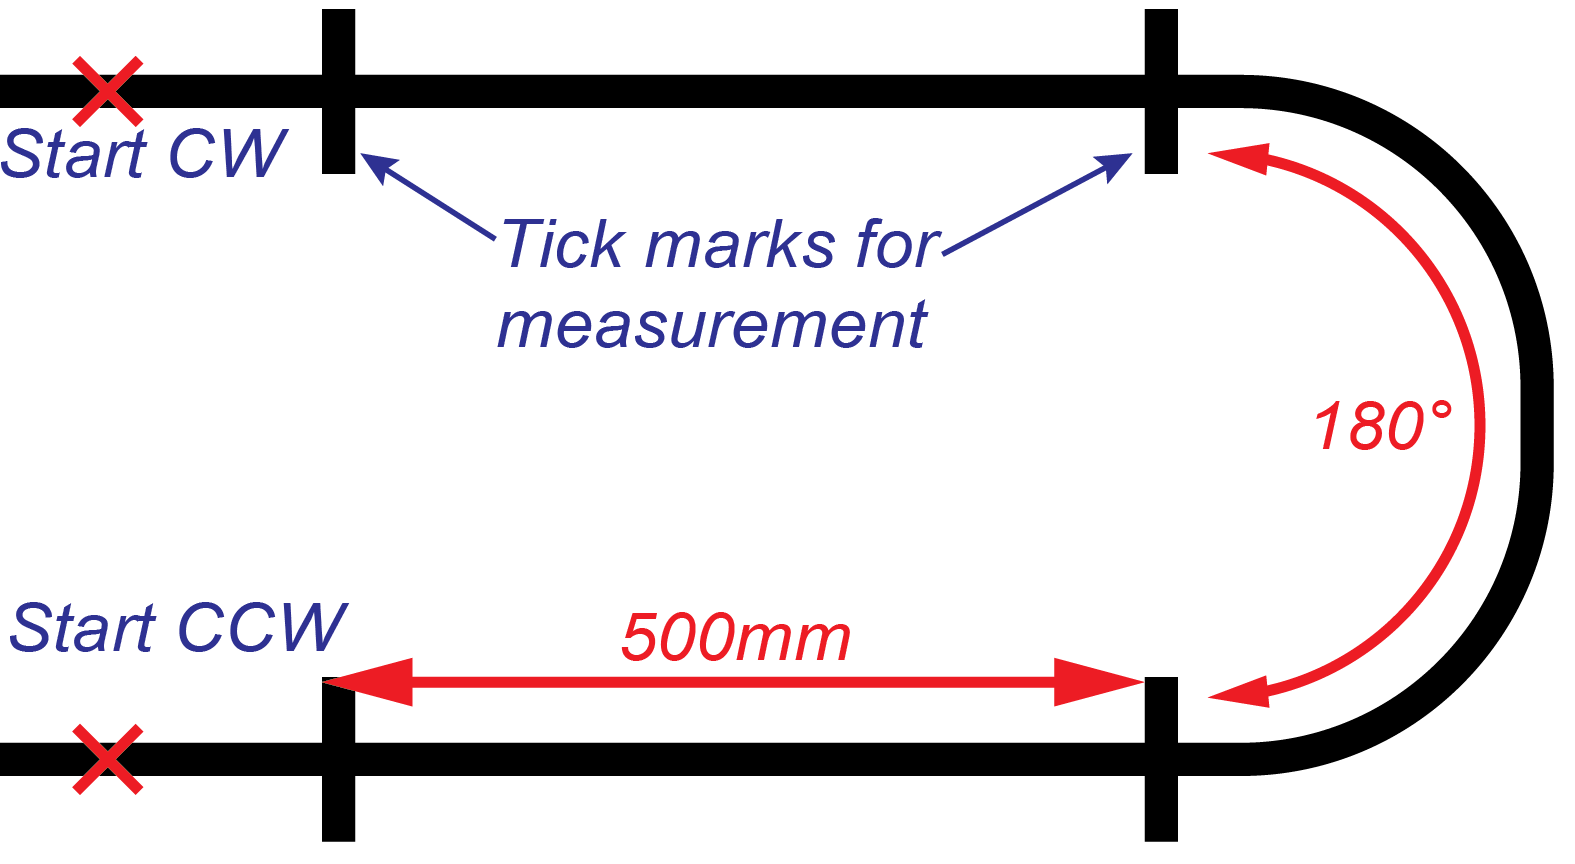
\includegraphics[width = 0.49\textwidth]{img/calibration_circuit.png}
    \caption{Calibration circuit diagram}
    \label{fig:calibration_circuit}
\end{figure}

The circuit comprises of a 0.5m straight line section, followed by a large radius 180-degree turn, followed by another 0.5m straight line section. 
At the beginning and end of each section, a perpendicular tick mark is printed which signals to the robot when to initiate and end the calibration procedure. 
The circuit is symmetrical, allowing for calibration in both directions to ensure that any differences between a clockwise and counter-clockwise calibration are averaged out.

The robot will complete the circuit by using the front line sensors to follow the line. 
The side line sensors detect the tick marks, signalling when to begin and end the calibration calculations, shown in Figure \ref{fig:calibration_circuit}. 
First, the robot completes the straight line section, measuring the distance between the tick marks based on the internal kinematics, comparing this to the known distance to calculate the wheel radii as seen in equation \ref{eq:linear}. 
In equations \ref{eq:linear} and \ref{eq:angle}, $R_i$ are the radii of the wheels, $C$ is the number of encoder counts per revolution, $d,\alpha$ are the circuit parameters: straight line distance and turn angle and $e_i$ are encoder counts for each wheel.

\begin{equation}
\label{eq:linear}
    R_i = \frac{C \times d}{2 \times \pi \times \Delta e_i}
\end{equation}

The robot then completes the turning section of the circuit, measuring the turn angle based on internal kinematics and comparing this to the known turn angle to calculate, with updated wheel radii, the wheelbase length $L$, as seen in equation \ref{eq:angle}.

\begin{equation}
\label{eq:angle}
L = \left|\frac{\pi \times (\Delta e_0 \times R_0 - \Delta e_1 \times R_1)}{\alpha \times C}\right|
\end{equation}

Upon completion, the robot will enter a state in which it repeatedly prints these new values to the serial monitor where they can be recorded. These values will then be updated manually in the kinematics of that robot before further testing.

To verify that the calibration algorithm measures the differences in key dimensions of the robot correctly, a robot with one tyre removed and then the same robot with wheels levered apart (to increase the wheelbase) is tested on the calibration circuit after each of these alterations (the tyre is replaced after the first test). The results in Table \ref{tab:verify}, show that the algorithm correctly identifies differences between key robot dimensions.

\begin{table}[h!]
\centering
\caption{Algorithm verification results}
\label{tab:verify}
\resizebox{\columnwidth}{!}{%
\begin{tabular}{l|c|c|c}
                   & R0 & R1 & L \\ \hline
Wheel removed      & \textbf{14.03}       & 16.23       & 42.39      \\ \hline
Wheelbase extended & 16.17       & 16.20       & \textbf{43.56 }    
\end{tabular}%
}
\end{table}

\vspace{-1.5cm}
% \begin{algorithm}

% \caption{Calibration Method} 
%     \label{algo:calibration}
% \textbf{Input:} Line sensor readings left to right:  linesensor[0,1,2,3,4], known length \textbf{and} angle \\
%  \textbf{Output:} Array of dimensions, $R_0,R_1,L$\\

%     \begin{algorithmic}
%         \State State = 1
        
%         \State \textbf{Update state:}
%         \If{State = 1
%         \textbf{and} linesensor[0] \textbf{and} linesensor[4]}
%             \State State = 2
%         \ElsIf{State = 2 \textbf{and} \textbf{not} linesensor[0] \textbf{and} \textbf{not} linesensor[4]}
%             \State Update encoder counts
%             \State State = 3
%         \ElsIf{State = 3 \textbf{and} linesensor[0] \textbf{and} linesensor[4]}
%             \State Calculate $R_0, R_1$ \textbf{or} $L$ 
%             \State State = 4
%         \EndIf\\
        
%         \State \textbf{State Actions:}
%         \If{State = 1 \textbf{or} State = 2 \textbf{or} State = 3}
%             \State Follow line
%         \ElsIf{State = 4}
%             \State Stop motors
%             \State Print $R_0,R_1,L$
%         \EndIf
%     \end{algorithmic}
% \end{algorithm}

\section{Experiment Methodology}\label{sec:experiment_method}

% \begin{itemize}
%     \item Run baseline accuracy tests for a number of robots. (linear distance and square error)
%     \item Run the calibration procedure to identify new dimensions for the robot.
%     \item Test the calibrated robots on the same set of accuracy tests.
%     \item Identify if there is an improvement.
% \end{itemize}

\subsection{Overview of Method}

The baseline, calibration and post-calibration tests were conducted on 3 different robots to investigate the variation between robots. 

First, the linear and orientation tests are completed on un-calibrated robots, using the default dimensions found on the robot data sheet \cite{pololu_guide} (shown in Figure \ref{fig:dimensions}), to establish a baseline set of results. 
The linear distance test is run ten times for each robot, documenting the error on each run. 
The orientation test (UMBmark) involves two laps around the square track, completed five times in each direction; clockwise and counter-clockwise.
Both orientation and position error from the origin on completion of the orientation test are recorded.

Each robot is then calibrated using the calibration circuit and calibration algorithm. 
The resulting robot dimensions from 10 repeat calibrations are recorded (for 5 in each direction).
The calibrated mean values for each wheel radius and wheelbase length are updated in each of the robot's kinematic models. 

Finally, each robot is re-tested on the original linear and orientation error tests in an identical manner to the baseline tests. 

\subsection{Discussion of Variables}

\begin{itemize}
    \item \textbf{Controlled Variables}: 
    For each test, the \emph{distance} and number of \emph{laps} are kept constant. 
    Each robot runs the same test code, using the same kinematic model, motor and heading PID controllers. 
    The target \emph{speed} of the robot is kept at 75mm/s, with a maximum acceleration set to ensure minimal wheel slip.
    Furthermore, \emph{ambient lighting} is kept constant due to its influence on the readings from the IR line sensors. 
    New, fully charged batteries are used for each set of tests.
    \item \textbf{Independent Variable}: 
    The independent variable is the robot itself. 
    As the experiment relies on autonomous measurement by the robot, the only changing variable will be the robot, and as a result the robot dimensions - $R_0, R_1, L$. 
    The method aims to observe a measurable difference in these parameters between robots and use this to explain any improvements in system accuracy after calibration. 
    \item \textbf{Dependent Variable(s)}: this experiment aims to measure the accuracy of the robots before and after calibration. The metrics used for quantifying the accuracy are the linear error for linear tests, orientation error and Euclidean distance error on return-to-home on the orientation test.
\end{itemize}

\subsection{Discussion of Metric(s)}

The calibration process aims to measure:
\begin{enumerate}
    \item the radii of the wheels,
    \item the width of the wheelbase,
\end{enumerate}
for each robot from the default values found in the data sheet.
The effect of calibration on the following variables will be measured to quantify the results:
\begin{enumerate}
    \item Linear error and p-value for error change
    \item Orientation error and p-value for error change
    \item Absolute position error and p-value for error change
\end{enumerate}

The linear error is used as it demonstrates the error from overshoot (positive error) and undershoot (negative error) due to incorrect wheel radius values $R_0, R_1$. This metric isolates the impact of wheel radii as the test is conducted on a straight line section and the wheelbase length $L$ does not impact the result, as seen in equation \ref{eq:linear}.

The orientation error is quantified with the error in angle on return to the origin. This error is an accumulation of the orientation errors during the test meaning that this metric provides an estimate of the systematic orientation error.
The orientation error, given correct wheel radii (as found in the first part of the calibration), isolates the impact of the wheelbase width $L$ allowing this metric to measure the effect of that variable on robot accuracy.

Finally, the Euclidean position error encompasses an overall odometry systematic error found for each robot. This provides an overall measure of robot accuracy and precision. The spread of error corresponds to the overall precision and the mean values correspond to the overall accuracy. 
This metric and both of these observations provide a clear comparison point for robot performance before and after calibration.


\section{Results}\label{sec:results}


The results of the tests before and after calibration are shown in this section, comparing the change in metrics for each of the three robots. 
A paired t-test has been used to assess the significance of the results for each robot. A paired t-test is selected as the variance of results before and after calibration is not assumed to be equal as the calibration could impact this. The tests are performed at a 5\% significance level.

\subsection{Measured dimensions}
\begin{figure}[h]
    \centering
    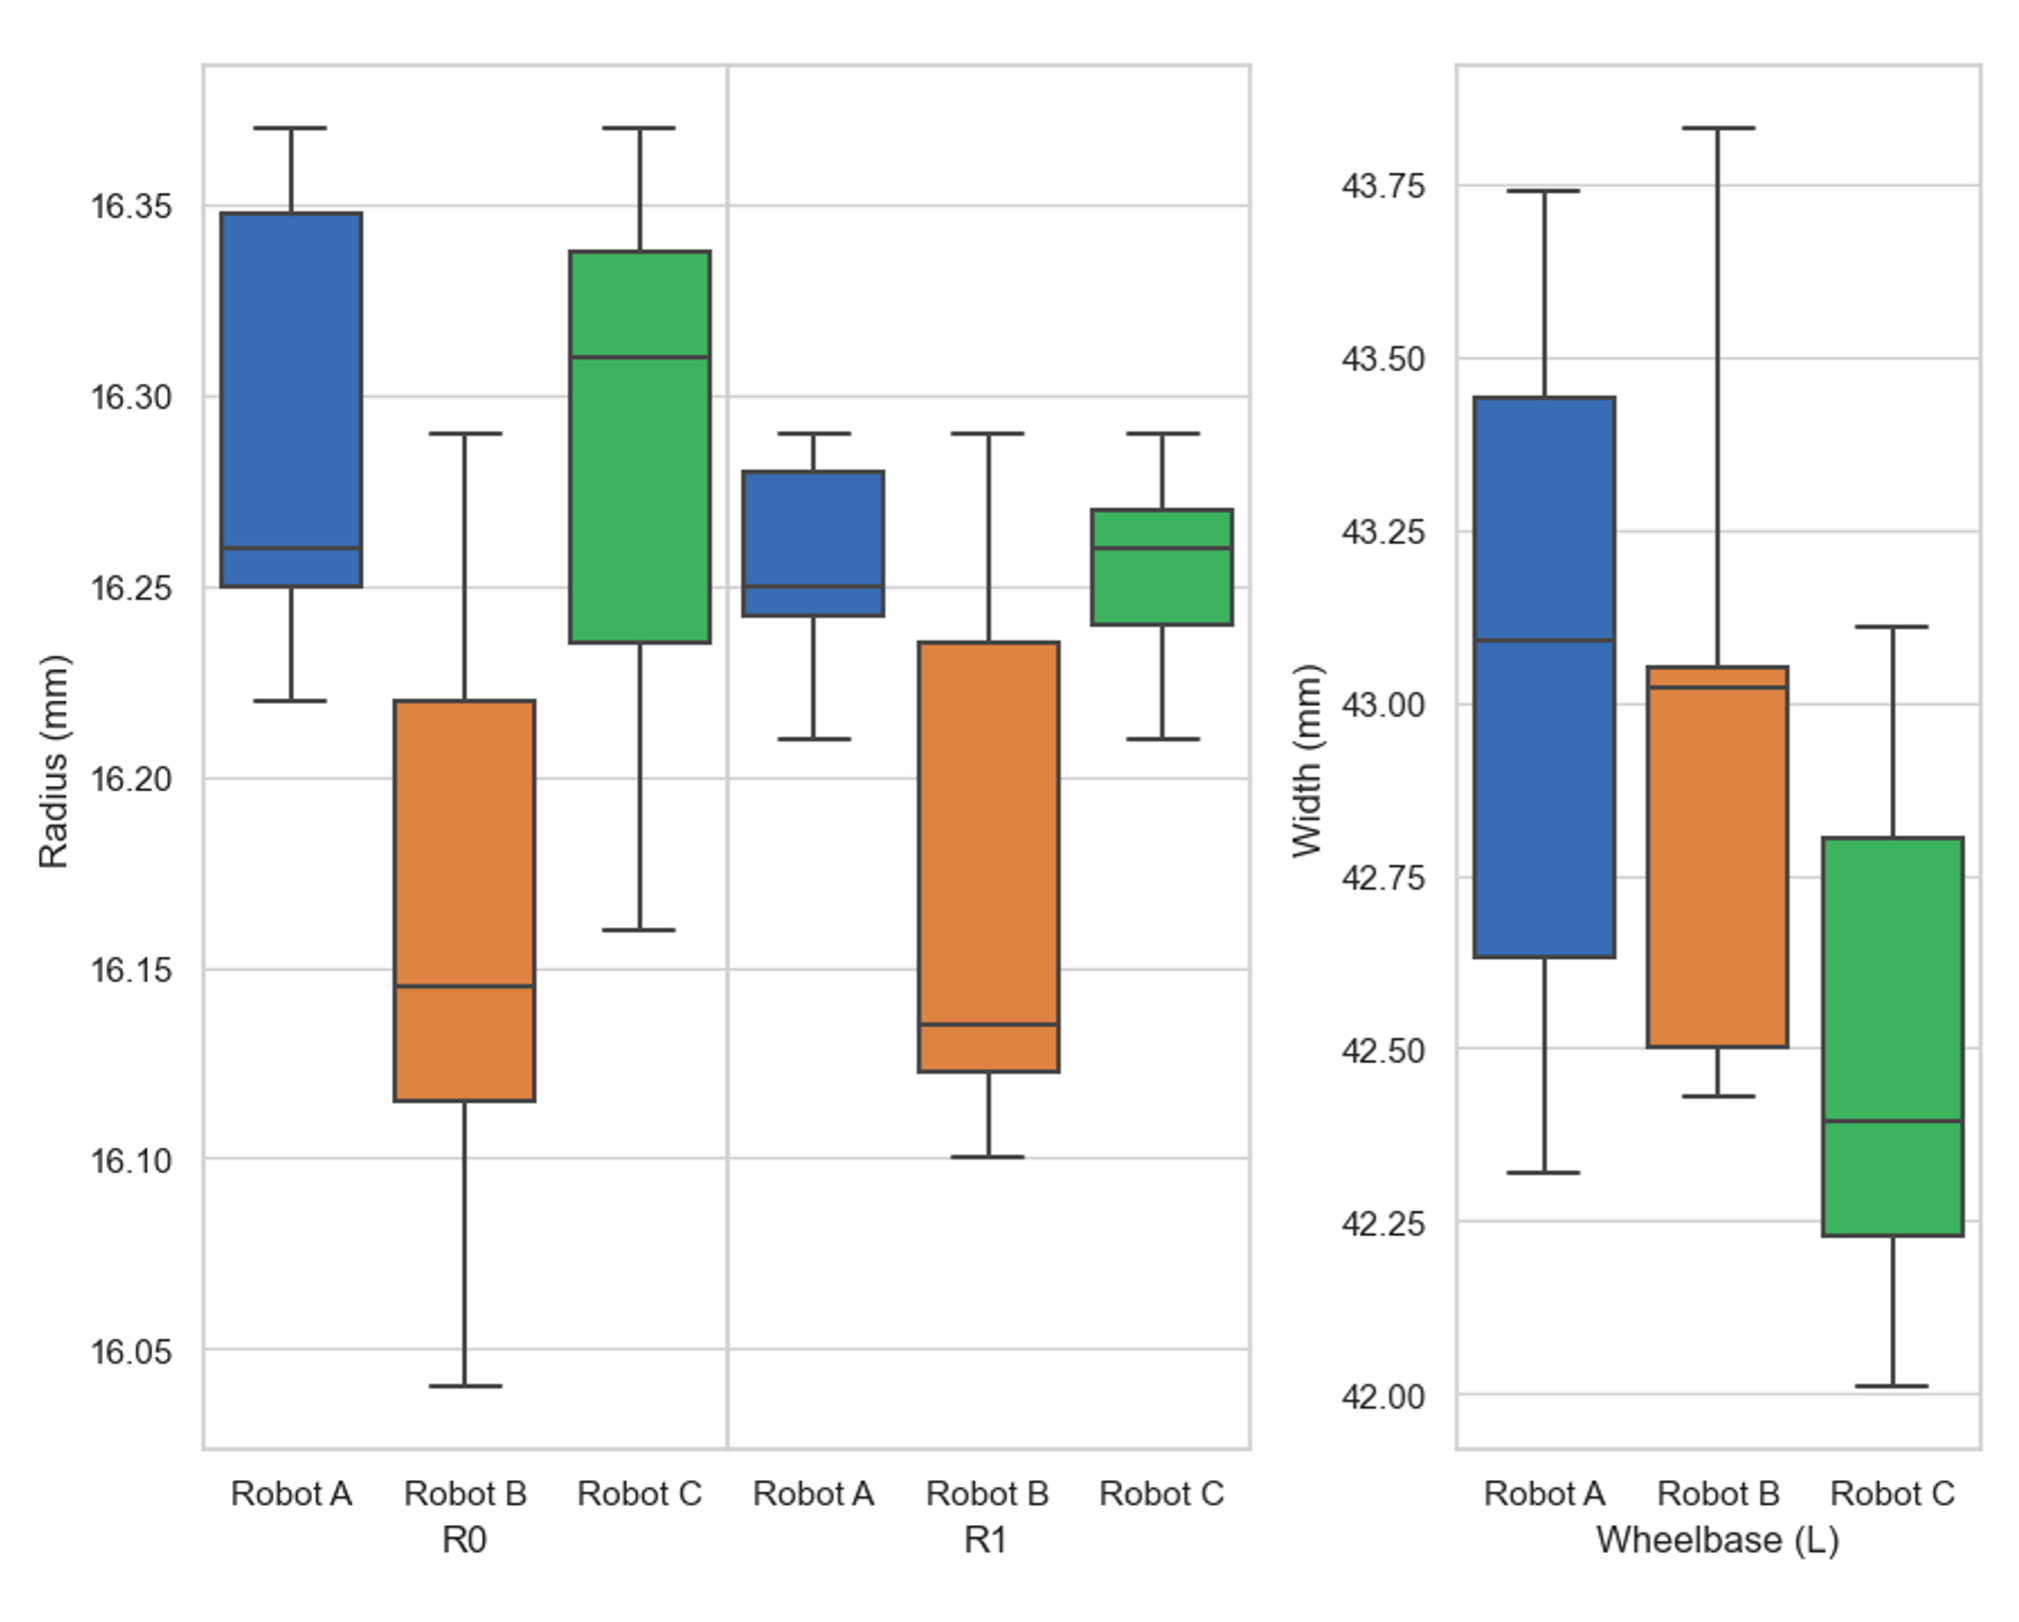
\includegraphics[width=.5\textwidth]{img/r0r1l.png}
    \caption{Measured key dimensions}
    \label{fig:r0r1L}
\end{figure}


The dimensions measured by the calibration method for each of the three robots are shown in Figure \ref{fig:r0r1L}. 
Although measurable, the difference between dimensions (R0, R1 and L) of any of the robots is not statistically significant ($n = 10$, two-tail, $p > 0.05 $) for any pairing. 
The median wheel radius is measured as 16.25mm rather than the data sheet dimension of 16mm. 
Similarly, the median wheelbase is measured as 42.87mm rather than 42.7mm.

\begin{figure*}[h!]
    \centering
    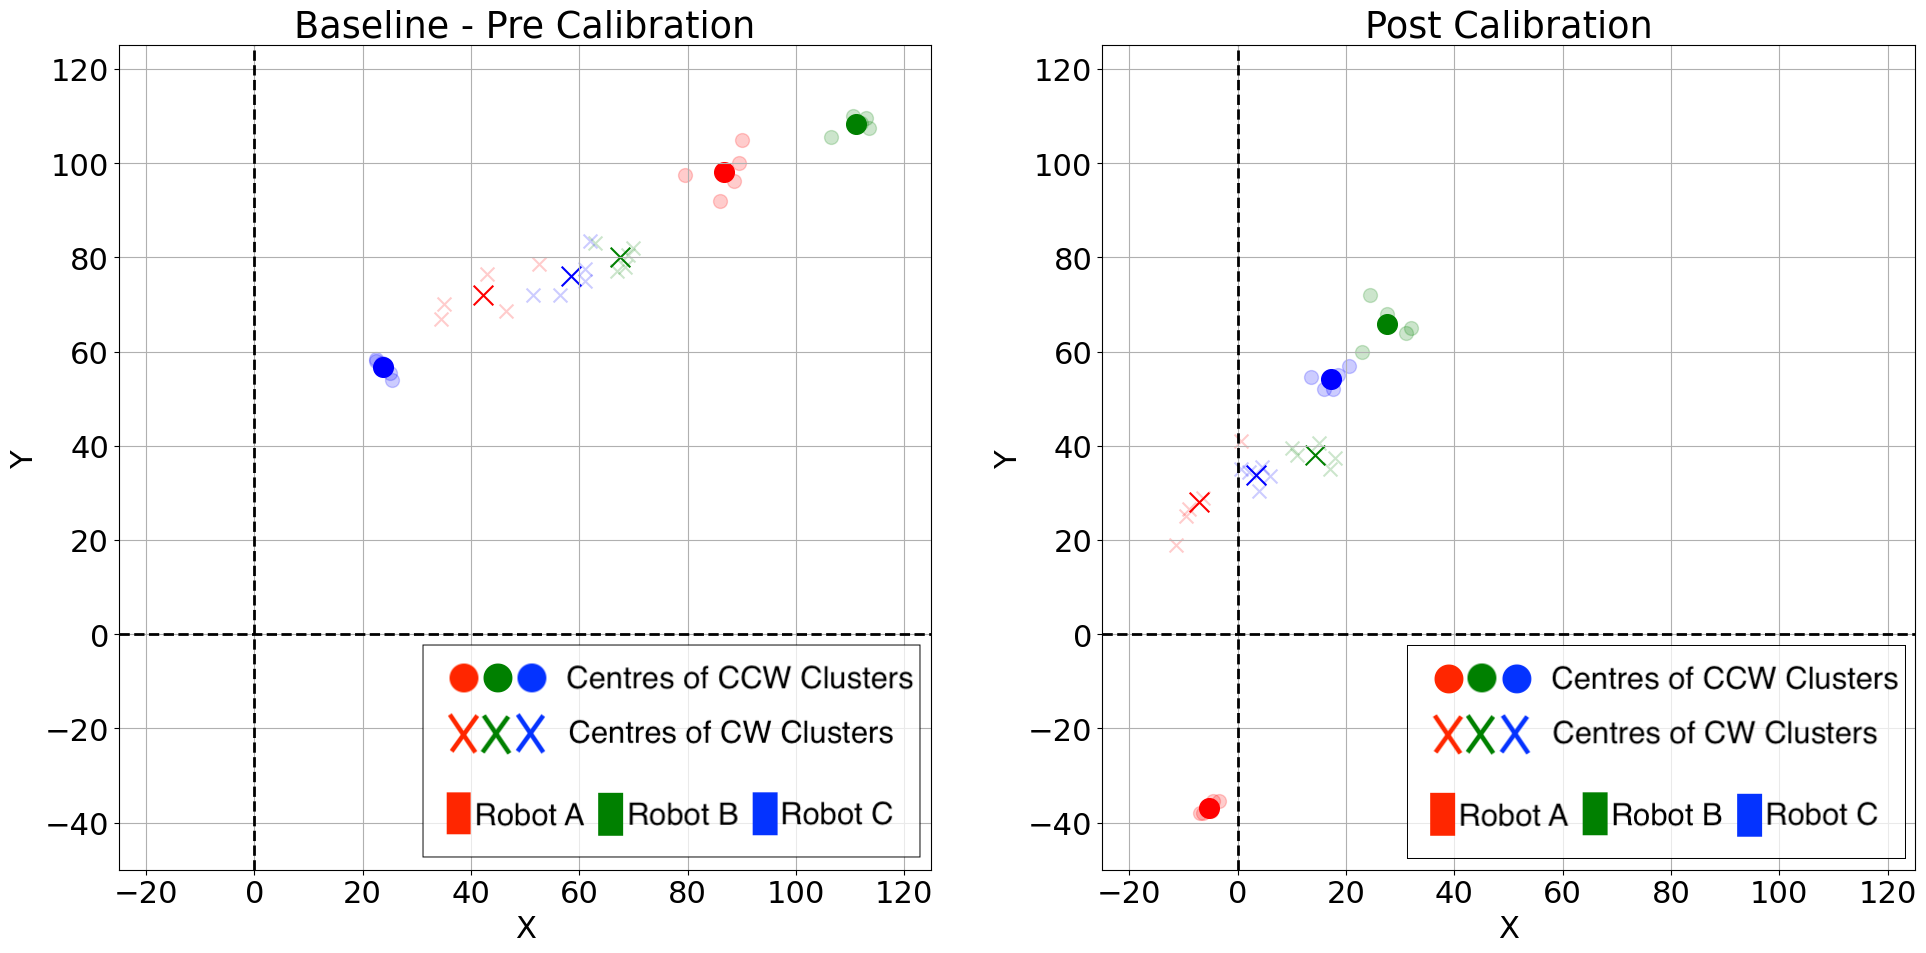
\includegraphics[width=.95\textwidth]{img/xy_pre_post_2.png}
    \caption{Return to home position relative to the origin for all three robots in the clockwise and counter-clockwise direction. The darker marks show the mean location for each cluster.}
    \label{fig:xy_scatter}
\end{figure*}

\subsection{Linear accuracy}


The first test compared the results of the linear accuracy measurement of the three robots. 
Pre-calibration the three robots all undershoot by varying amounts, while post-calibration the robots' absolute mean error is smaller by an average of 8.2mm, showing a statistically significant decrease in error with an average paired t-test ($n = 10$, one-tail, $p = 0.004$). The distribution of errors for the three robots is shown in Figure \ref{fig:linear}.

\begin{figure}[h]
    \centering
    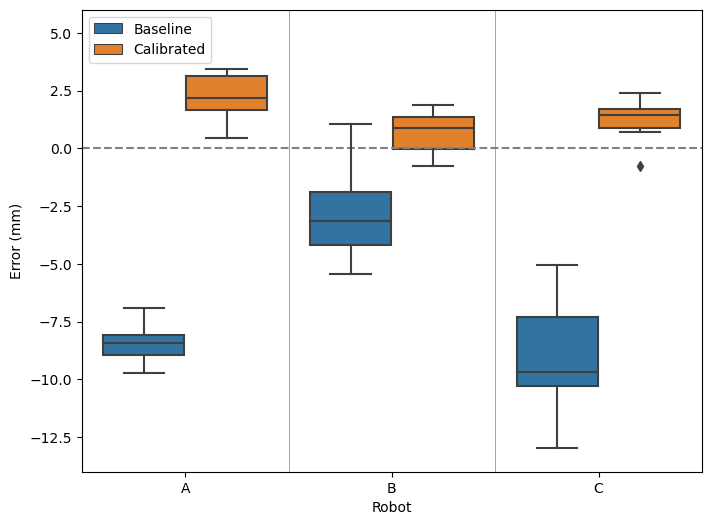
\includegraphics[width=.49\textwidth]{img/linear_pre_post.png}
    \caption{Linear error over 0.5m before and after calibration}
    \label{fig:linear}
\end{figure}

\subsection{Orientation accuracy}

The orientation error calculated from the UMBmark test is plotted in Figure \ref{fig:orientation}. The distributions appear to show a clustering of results based on the direction of travel around the test circuit in the baseline results.

A paired t-test reveals that there is significant clustering ($n = 5$, one-tail, $p < 0.05$) for all robot test results apart from the post-calibration result of Robot A ($p=0.051$). The test also reveals an average increase in p-value between pre-calibration and post-calibration of over two orders of magnitude (143.9) suggesting that the clustering reduces as a result of calibration. 

\begin{figure}[h!]
    \centering
    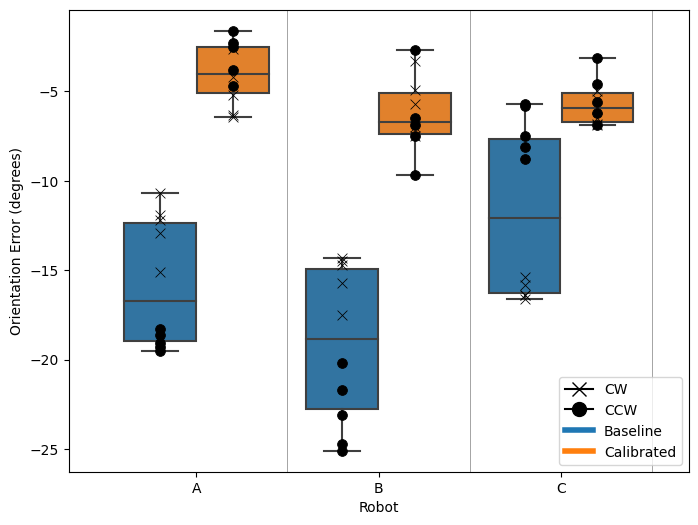
\includegraphics[width=.49\textwidth]{img/orientation_error.png}
    \caption{Orientation error before and after calibration}
    \label{fig:orientation}
\end{figure}



Additionally, Figure \ref{fig:orientation} shows a reduction in orientation error between the baseline and calibrated measurements for all robots. The difference is statistically significant ($n = 10$, one-tail, $p < 0.05$) for all robots with p-values $p=1.5\times10^{-6}$, $p=2.9\times10^{-9}$ and $p=0.01$ respectively. 

Figures \ref{fig:xy_scatter} and \ref{fig:xy_box} show the pre and post-calibration position error from the UMBmark tests. 
The cluster centres are marked and separated by the test direction (CW or CCW).
Figure \ref{fig:xy_box} shows the distribution of linear Euclidean distances from the origin at the end of UMBmark tests, indicating a decrease in position error and standard deviation of errors. 
The average standard deviation was reduced by 10mm to 14mm after calibration.
For all robots, the return to home error paired t-test found the difference between means to be significant ($n = 10$, one-tail $p < 0.05$). 

\begin{figure}[tbh!]
    \centering
    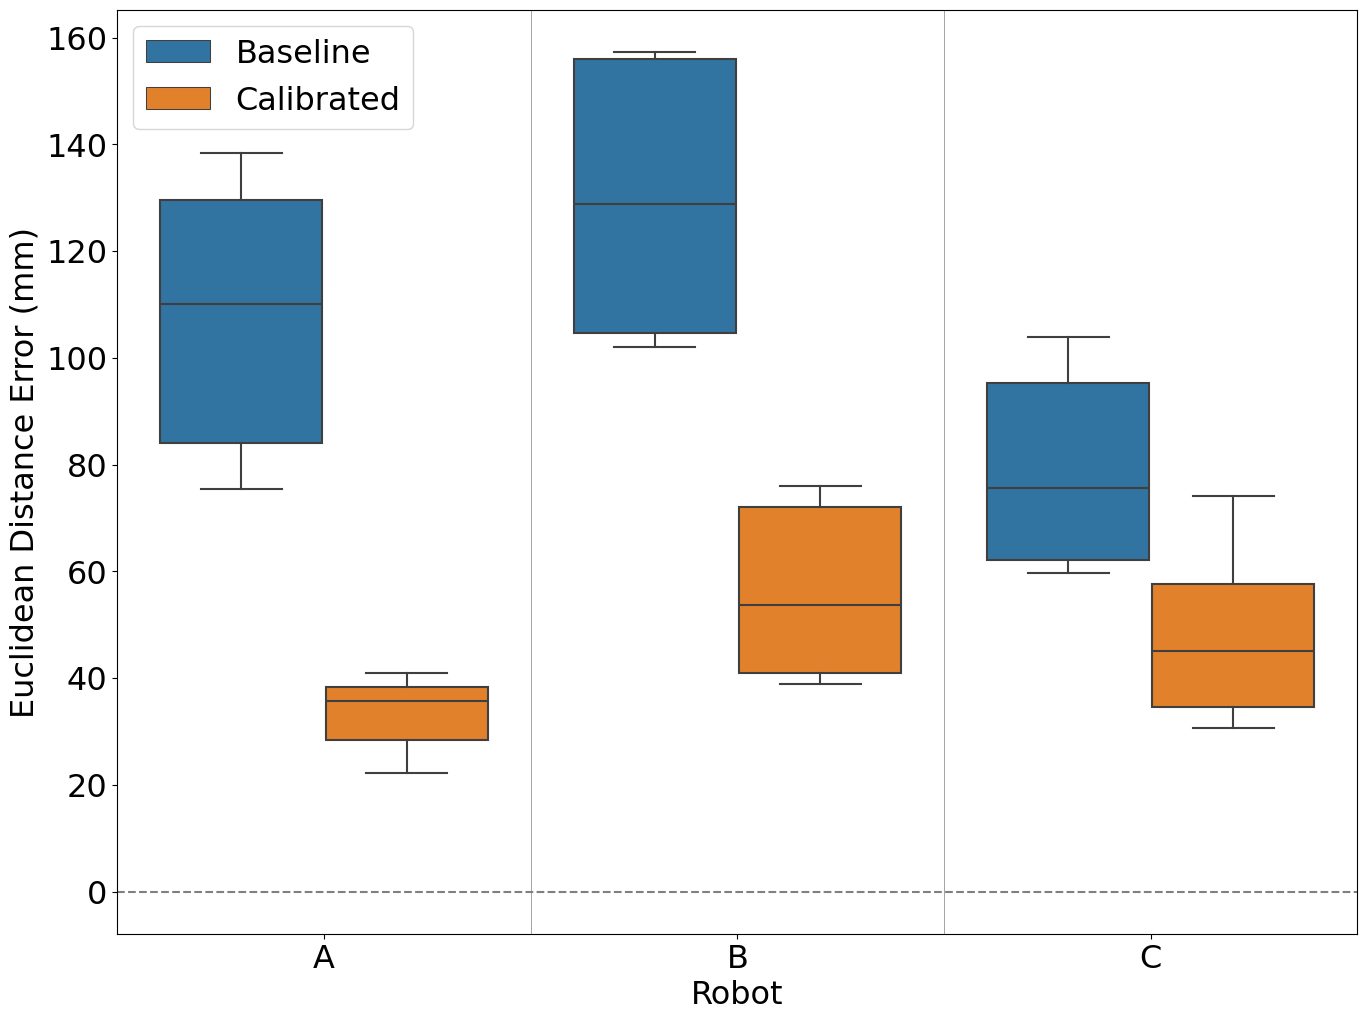
\includegraphics[width = 0.48\textwidth]{img/xy_error_boxplot.png}
    \caption{The Euclidean distance error in return to home position before and after calibration.}
    \label{fig:xy_box}
\end{figure}




\section{Discussion and Conclusion}\label{sec:discussion_conclusion}

The results of this study are used to discuss the original hypothesis:

% Make a discussion of what your results showed - whether this supported or refuted your hypothesis. Try not to respond to your hypothesis as if you were right or wrong, or successful or unsuccessful.  Instead, evaluate your hypothesis for whether it helped you to learn something - was it a good question or prediction to make?  Was it useful in this way?  If not, in what way does the hypothesis need adjustment, to guide future experiments? 
% In your discussion, use this as another opportunity to demonstrate/evidence your understanding. Try to avoid stating the obvious - instead, use analysis/evaluation/synthesis to show that you understand \emph{how} and \emph{why} you saw the results you did. 

\begin{quote}
    \emph{
    The authors hypothesize that variances in wheel diameter and wheelbase width significantly affect the odometry accuracy of the Pololu 3Pi+ robot.
    This experiment predicts that a calibration circuit and method using onboard sensors can automatically measure the wheel radii and wheelbase.
    By applying this calibration, we anticipate a measurable improvement in odometry accuracy through a reduction in systematic errors when compared to performance using the default dimensions from the datasheet.}
\end{quote}

Analysis of the calibration data reveals some variability in the key dimensions across the tested robots, which is possibly caused by manufacturing and assembly tolerances. 
Although there are measurable differences in dimensions between the robots, they did not reach statistical significance (p $>$ 0.05 for all comparisons). 
This indicates that while observable differences in key dimensions exist, they are not sufficiently large or consistent enough to be considered statistically reliable under the tested conditions.
These findings suggest that the current measurement accuracy and precision are inadequate to reliably differentiate these deviations. 
Improving the accuracy and precision of the calibration measurements is expected to reduce measurement variability, narrow confidence intervals, and result in smaller p-values, potentially increasing the statistical significance of these findings.\\

The median values for the wheel radius and wheelbase (16.25mm for radius instead of 16mm, and 42.87mm for wheelbase instead of 42.7mm) suggest that the default dimensions could be adjusted to better reflect the actual measurements found during calibration. 
These adjusted values could potentially improve the baseline settings of future robots, improving their odometry accuracy out of the box.

The hypothesis predicts improvements in both linear and orientation accuracy through calibration.
The linear error is lower post-calibration for all robots, due to a more accurate wheel radius, supporting the hypothesis that automatic calibration can improve the system's linear accuracy. 

The clustering seen in the pre-calibration results for the CW and CCW tests is likely due to a mismatch in wheel sizes, and wheelbase width differing from the nominal.
A mismatch in wheel radii causes the robot to drive along a curved path, while an incorrect wheelbase causes an orientation error when turning 90 degrees.
These errors add up when the robot completes laps of the square in one direction, and cancel out when completing the laps in the opposite direction.
This combination of systematic errors causes the clustering separation between CW and CCW return positions seen in Figure \ref{fig:xy_scatter}.
In extreme cases, testing in only one direction can appear to show a robot with accurate odometry (where systematic errors cancel out), however, when the robot completes the task in the opposite direction it is seen to have a much lower accuracy.
The clustering separation is significantly reduced post-calibration, indicating that the calibration effectively identifies and corrects the sources of these systematic odometry errors. \\

Very small deviations in key dimensions such as wheel radii and wheelbase widths, often less than 0.5mm, are shown to significantly impact the accuracy and precision of the robot's odometry. 
Typically, these small variations are beyond the measurement capability of standard rulers available to most users, meaning that the proposed method of calibration achieves better odometry accuracy than hand measurement techniques.
Trial and error techniques can achieve better accuracy but are more time-consuming and prone to user error, making it impractical for applications with multiple robots or swarms.

Measuring the wheel radius accurately using metrology tools, such as vernier calipers, presents difficulties due to the compressibility of the rubber, and obstacles such as the wheel housing. 
The proposed calibration method may prove particularly beneficial for the automatic measurement of the effective wheel radii of robots equipped with pneumatic tyres.
In such cases, the effective wheel radius may vary based on the weight of a payload or changes in tyre pressure caused by changes in ambient temperature. 
These factors complicate the direct measurement of wheel radii through conventional methods.
Instead, measuring the wheel radii dynamically while the robot is in use, could offer a more reliable and efficient solution for maintaining accurate odometry in robotic applications where wheel deformation is a concern, such as warehouse robotics or assembly lines.

\paragraph{Limitations}

The findings in this report are limited by a number of factors related to systematic and non-systematic errors and the assumptions used for the control of the robot. 

There are a number of potential sources of systematic error that are assumed to be negligible in this investigation.
These are the gearbox slip, misalignment of wheels and the limits of the encoder resolution. 
There is significant evidence in literature that the impact of these factors is much less than of those investigated in this study \cite{UMBmark}. 
However, these factors could be producing some of the random error seen in the results, assuming these errors are negligible limits the accuracy of calibration. 

Non-systematic errors have been identified and attempts made to mitigate them, however, these errors still contribute to randomness in the distribution of results. 
Their impact is mitigated by taking a large number of measurements. 
Potential non-systematic errors include wheel slip, changes in lighting for line sensor reading accuracy, and surface irregularities. 
These errors are controlled by limiting robot speed and acceleration, consistently controlling lighting, and using a clean, flat surface respectively. 
However, due to the high measurement resolution required for accurate odometry, even minor environmental variations can induce errors.

Limitations of the robot control implementation include the kinematic model and motor control. 
The differential drive kinematic model assumes that wheel revolutions are directly proportional to linear distance, neglecting wheel slippage and mechanical differences in the drive \cite{odometry}. 
It also approximates arcs with straight line segments, limiting the accuracy of the displacement calculation by the update period. This is mitigated through the use of high-frequency kinematic updates and slow driving speeds, so straight line segments closely approximate arced paths.
However, this could be improved further by using an arc-based kinematic model.

Additionally, the system uses a motor and heading PID controller tuned for one of the robots, assuming the same response for all robots.
The calibration circuit requires smooth line-following behaviour, without significant heading oscillation.
Variations in the system response between robots could lead to increased wheel slip or worse heading control, resulting in larger orientation errors on some robots. 
To reduce the impact of a controller a larger test distance could be used, thereby allowing more time for a heading response to settle in the case of the orientation error test.


\paragraph{Future work}

Further work should look to improve the calibration accuracy, which is currently limited by unaccounted-for systematic errors, non-systematic errors, the line sensor accuracy and the accuracy of the printed calibration circuit. 
While mitigations for the systematic and non-systematic errors have been described above, a key area for further improvement is the line sensor accuracy. 
These sensors are the only form of feedback the robot receives from the environment, and while mitigation for threshold errors is described in Figure \ref{fig:linesensor}, the sensor readings are still subject to some random variation that can impact the calibration accuracy.
Future accuracy improvements could be achieved by avoiding the limitations of the line sensors, and using an alternate form of measurement, with external camera IR reflectors, or laser measurement, but this will increase cost and complexity.
Sensor fusion using the built-in inertial sensors and magnetometer could also be investigated to improve accuracy. 

A larger printed calibration circuit, making use of larger turn angles or combinations of turns in both directions, could further improve the accuracy of calibration measurements as the percentage error would decrease.

Finally, for practical application, the process of dimension update should be automated. This will ensure that the time saving of calibration is much higher, and allow it to be integrated into general robotic tasks, for example as part of autonomous swarms.


\bibliographystyle{ieeetr} 
\bibliography{biblio}


\end{document}
